\documentclass[a4paper]{scrreprt}

\usepackage[ngerman]{babel}
\usepackage[utf8]{inputenc}
\usepackage[T1]{fontenc}
\usepackage{ae}
\usepackage[bookmarks, bookmarksnumbered]{hyperref}
\usepackage{tabularx}
\usepackage{graphicx}
\usepackage{csquotes}
\usepackage{verbatim}
\usepackage{float}
\usepackage[nonumberlist, toc, section]{glossaries}
\usepackage[german]{fancyref}

\setcounter{secnumdepth}{4}

\begin{document}

\title{Implementierungsdokument CS:Select}
\author{Luca Springer, Alexander Linder, Julian Dinh, Nicholas Bieker,\\ Bendix Sonnenberg}
\maketitle

\tableofcontents


\chapter{Einleitung}

In diesem Dokument beschäftigen wir uns mit der Implementierungsphase unseres Projekts CS:Select. Dabei befassen wir uns insbesondere damit, welche Kriterien wir aus unserem Pflichtenheft umgesetzt haben und welche Änderungen sich zu unserem Entwurf ergeben haben. Da das Front-End im Entwurfsdokument nur sehr oberflächlich behandelt wurde, gehen wir nun nochmal genauer darauf ein, wie dieses gestaltet wurde. Außerdem stellen wir dar, wie die Implementierung zeitlich abgelaufen ist und welche Frameworks und Bibliotheken wir dabei benutzt haben. Schlussendlich gibt es einen einen Überblick über die bereits vorhandenen Unit-Tests.

\hspace{1cm}

Generell kann das Projekt in die Bestandteile Front-End und Spiel-Server aufgeteilt werden. Für das Front-End haben wir dabei mit HTML, CSS und JavaScript gearbeitet, während der Spiel-Server in Java geschrieben ist. Dieser beinhaltet ein Datenbank-Paket, welches wir mithilfe von mySQL implementiert haben. Das Front-End und der Spiel-Server kommunizieren über eine von uns definierte API.

\hspace{1cm}

Ein grundlegender Gedanke unserer Implementierung war es, möglichst wenige Daten im Arbeitsspeicher und möglichst viele in unserer Datenbank zu halten, um das Erhalten des Server-Status beim Beenden und bei einem möglichen Absturz sicherzustellen und Inkonsistenzen zu verhindern. Das wurde über die Kommunikation verschiedener Klassen und Objekte mit der Datenbank über eigene Adapter erreicht. 

\hspace{1cm}

Insgesamt haben wir so X Commits getätigt und es sind X Pakete, Y Klassen sowie Z Codezeilen entstanden. %Konkrete Werte


\chapter{Implementierte Kriterien}

\section{Muss-Kriterien}
Alle Muss-Kriterien aus dem Pflichtenheft wurden bei der Implementierung berücksichtigt und alle zugehörigen Funktionellen Anforderungen sind implementiert.


\section{Kann-Kriterien}
Die folgenden Kann-Kriterien sind inklusive aller zugehörigen Funktionellen Anforderungen implementiert:

\begin{itemize}
\item Erweiterte Nutzerverwaltung (E-Mail-Adresse und Passwort ändern sowie Passwort zurücksetzen)
\item Zusätzliche Funktionen für den Organisator in der Übersichts-GUI (Spiele vorzeitig beenden und beendete Spiele aus der Übersicht löschen)
\item Speichern und Laden von Spieleinstellungen bei der Spielerstellung
\item Zusätzliche Optionen für den Spieler im Spiel (Runde überspringen, Merkmal als unwichtig markieren)
\item Gamification-Elemente Leaderboard, Achievements, Daily-Challenges und Streaks
\item Bedienungshilfen %???
\item Internationalisierung (Sprache im Browser ändern, englisches Sprachpaket)
\end{itemize}

\hspace{1cm}

Weitere Kriterien sind teilweise implementiert, d.h. manche zugehörige funktionale Anforderungen sind implementiert, andere hingegen nicht:

\subsection{Zusätzliche Funktionen zur Verwaltung des Spiel-Servers}
Zusätzliche Funktionen zur Verwaltung des Spiel-Servers: Dadurch, dass alle Daten in unserer Datenbank gespeichert werden und nicht im Arbeitsspeicher gehalten werden, wird der Zustand des Spiel-Servers auch bei einem Neustart erhalten. Spiele und Organisatoren können direkt aus der Datenbank gelöscht werden. Die Kommunikation eines Administrators mit dem System über eine Kommandozeile ist dagegen nicht möglich und es gibt auch keinen Dialog beim Aufsetzen des Servers, da dafür die Config-Datei genug sein sollte.  

\subsection{Verbesserung der Merkmalsbereitstellung für ein Spiel}
Solange das möglich ist, wird das Anzeigen von gleichen Merkmalskombinationen in einem Spiel vom System verhindert. Bis auf diese Einschränkung erfolgt das Erzeugen der angezeigten Merkmalskombination jedoch zufällig.


\subsection{Unterstützung von mehreren Plattformen}
%???


\hspace{1cm}

Das letzte Kann-Kriterium, weitere Spielmodi, wurde dagegen aus Zeitgründen und aufgrund von einem Mangel an sinnvollen Ideen nicht umgesetzt.

\chapter{Änderungen zum Entwurf}
%Andere Gliederung?
\section{API}

\section{User}

\section{Database}
\begin{itemize}
    \item Neue Param-Klassen zum parametrisierten Aufruf von Mysql-Prepared-Statements wurden hinzugefügt
    \item Die registerPlayer/Organiser Methoden heißen nun createPlayer/Organiser und der eigentliche Registrierungsprozess wurde ausgelagert
    \item FeatureSet Informationen werden nicht mehr in die DB geschrieben sondern verbleiben in der erhaltenen .json Datei auf dem Dateisystem
    \item Neue Oberklasse für alle Adapter (MysqlAdapter) hinzugefügt, die Hilfsmethoden zum einfacheren Zugriff auf die Datenbank bündelt
    \item Der DatabaseAdapter besitzt nun eine getPlayer(int id) Methode
    \item getPlayer/OrganiserSalt, getPlayer/OrganiserHash Methoden wurden hinzugefügt um Hash bzw. Salt von Spielern anhand ihrer Email laden zu können
    \item getPasswordSalt wurde dem UserAdapter hinzugefügt, da die Passwortprüfung ausgelagert wurde
    \item getActive/TerminatedGames wurden in den UserAdapter verlegt, da sowohl Player als auch Organiser diese Methoden benötigen
    \item Klasse PlayerStatsAdapter hinzugefügt um die PlayerStats in die Datenbank abzubilden
    \item getInvitedPlayers im DatabaseAdapter gibt nun eine Collection von E-Mail-Addressen als Strings statt Player-Objekte zurück, da eingeladene Spieler nicht notwendigerweise bereits in CS:Select registriert sein müssen
    \item addPlayingPlayer zum GameAdapter hinzugefügt um einzelne Spieler komfortabler hinzufügen zu können
\end{itemize}

\section{GameCreation}

\section{Game}
\begin{itemize}
	\item Der Datentyp für Zeitpunkte ist LocalDateTime anstatt Date.
	\item Features werden in FeatureSet als Set gespeichert, dementsprechend gibt die Methode getFeatures auch ein Set statt einer Collection zurück.
	\item Die Methode getFinished von Game heißt nun isTerminated, da sie kein Getter ist sondern die Terminierung überprüft.
	\item Die Methode getRounds von Game gibt Collection statt Liste zurück, da die Reihenfolge hier nicht relevant ist.
	\item Entsprechend dem Vorgehen bei den Usern wird auch beim Game über die Datenbank sichergestellt, dass evtl. verschiedene Objekte zum gleichen Spiel synchronisiert sind, deshalb sind die Attribute invitedPlayersEmails und numberOfRounds sowie die Assoziationen zum Spieler und zur Runde über die Datenbank realisiert.
	\item Die Klasse Termination hat Setter-Methode für das zugehörige Spiel.
	\item Die Rundennummer ist nicht relevant und wurde somit nicht implementiert, deswegen ändern sich auch die Signaturen der entsprechenden Fabrikmethoden der Spielmodi.
	\item Die Klasse GamemodeComposite hat nun eine getGamemode Methode.
	\item Die Methoden skip und selectFeatures der Klasse Round benötigen keine Feature-Objekte, sondern nur deren ID, deshalb wurde die Methodensignatur entsprechend geändert, genauso auch die Methode acceptInvite der Klasse Game mit der \newline PlayerID statt einem Objekt.
	\item Bei der provideFeatures-Methode ist die Reihenfolge der erzeugten Features relevant, deshalb ist hier nun der Rückgabetyp eine Liste statt einer Collection.
	\item Runden haben nun eine setGame Methode.
	\item Die Boolean-Rückgabewerte der Methoden invitePlayers, acceptInvite und declineInvite waren unnötig und wurden rausgenommen.
	\item Die delete-Methoden von TerminationComposite und GamemodeComposite wurden nicht benutzt und dementsprechend entfernt.
	\item Die Klasse Game hat nun eine checkDuplicateFeatureProvision-Methode, um sicherzustellen, dass in einem Spiel nicht die gleiche Merkmalskombination mehrfach angezeigt wird.
\end{itemize}

\section{Gamification}
\begin{itemize}
  \item Die Methode calculateScore im Gamification-Interface wurde zu finishRound umbenannt, da der Name zuvor irreführend war. Da PlayerStats dieses Interface implementiert, wurde dementsprechend auch dort die Methode umbenannt.
  \item Die Methode getPlayers vom Leaderboard gibt nun eine sortierte Map (LinkedHashMap) anstatt einer Liste zurück. Ein Spieler wird dabei auf die entsprechende anzuzeigende Punktezahl (je nach Sortierstrategie) gemappt. Daraus folgen ebenso Signaturänderungen in SortingStrategy und deren Unterklassen.
  \item Für die SortingStrategy im Leaderboard gibt es nun einen Getter.
  \item In der abstrakten Klasse DailyChallenge fällt die Methode resetDaily weg, da sie obsolet ist.
  \item Der Datentyp für das Datum einer DailyChallenge ist LocalDate anstatt Date.
  \item Der Setter für das für das Datum einer Daily-Challenge fällt weg, dieses wird im Konstruktor gesetzt.
  \item Der Aufbau von Achievements unterscheidet sich grundlegend vom Entwurf. Es gibt nun ein Enum AchievementType, welches alle Achievements
    enthält. Jede Instanz dieses Enums implementiert eine abstrakte Methode getState. Beim Aufruf der Methode checkProgress
    wird dann nun der Status des Achievements-Typs ermittelt und ein neues konkretes Achievement mit entsprechenden Attributen
    erzeugt (Schablonenmethode). Außerdem bietet das Enum weitere Methoden für die Namen bzw. Beschreibungen, welche im Front-End
    angezeigt werden (getName, getDescription) an. Die festgelegten Achievements aus dem Entwurf sind jedoch gleich geblieben.
  \item Die Klasse Achievement ist dementsprechend nicht mehr abstrakt. Konkrete Achievements werden in der checkProgress-Methode
    der Enum-Instanzen erzeugt. Außerdem existiert nun eine Referenz zum Enum AchievementType.
  \item Die verschiedenen Attribute, die die Klasse PlayerStats im Enwturfsdiagramm besitzt, werden nun in der Datenbank abgespeichert, damit diese
    einen eventuellen Serverabsturz überstehen. Daher erwartet der PlayerStats-Konstruktor nun einen PlayerStatsAdpater.
  \item Aufgrund der Umstrukturierung der Achievements exisitiert auch keine statische Liste aus Achievements in PlayerStats mehr.
\end{itemize}

\section{Sonstiges}
\begin{itemize}
    \item Configuration, MLServer und DatabaseAdapter jetzt Interfaces die von einer Injector Klasse ausgeliefert werden.
    Die jeweilige Implementierung wird durch ein Module-Objekt festgelegt, das die jeweiligen Implementierungen den Interfaces je nach Anwendungszweck zuordnet.
    \item DefaultConfiguration umbenannt zu ApacheCommonsConfiguration nach der genutzten Bibliothek
\end{itemize}

\chapter{Front-End}

\chapter{Frameworks und Bibliotheken}

\chapter{Zeitlicher Ablauf}
Die ursprüngliche Planung der Phase ist im folgenden Implementierungsplan als Gantt-Chart festgehalten:

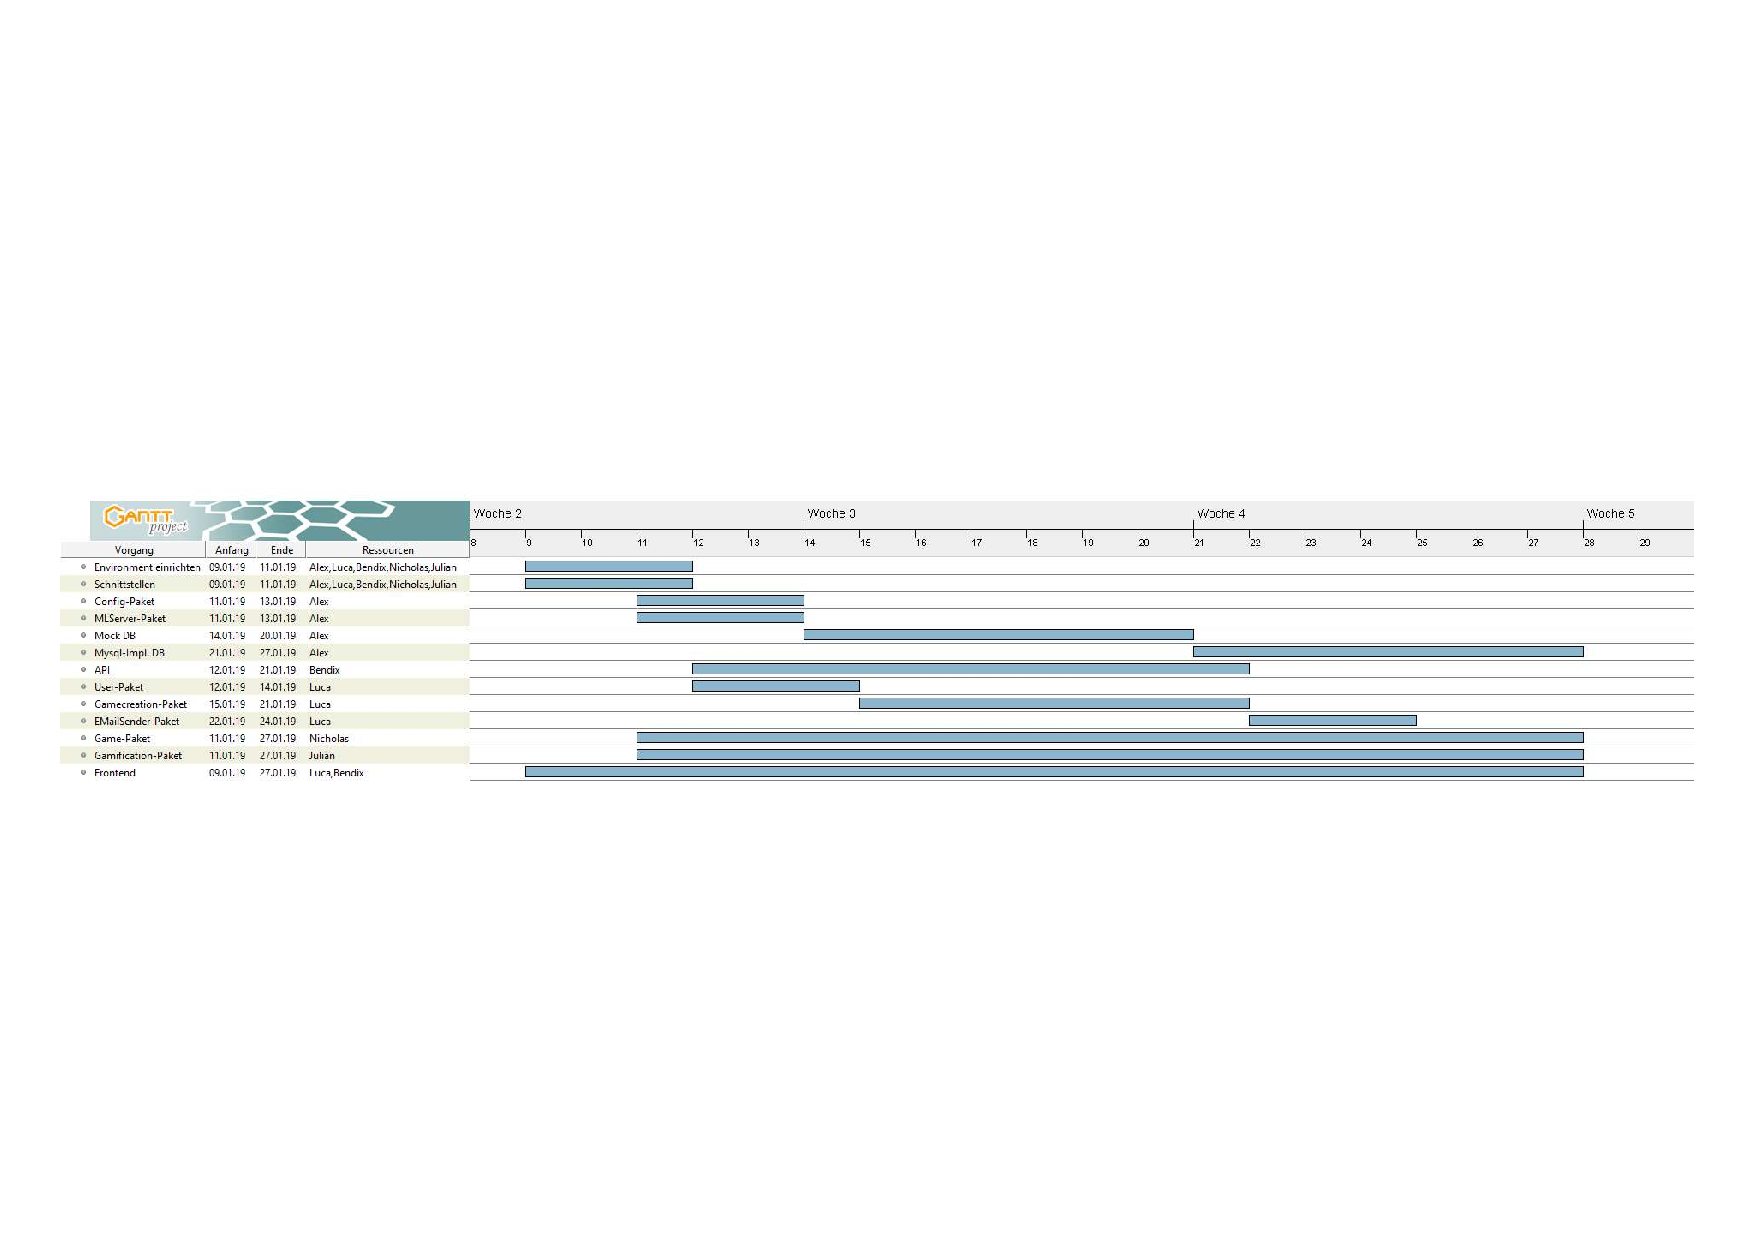
\includegraphics[width=\linewidth]{img/gantt.pdf} %in Anhang?

Dabei sollten aufgrund der Abhängigkeiten untereinander zunächst die kleineren Pakete und besonders das User-Paket fertiggestellt werden, die größeren Pakete Database, Game und Gamification sowie das Front-End waren dagegen länger eingeplant. Das ist auch soweit eingetroffen, auch wenn die letzten Schnittstellen erst ein wenig später als geplant vorhanden waren. Die ersten Pakete, also das Config-Paket, das ML-Server-Paket und das User-Paket waren bis auf einzelne Methoden im Zeitplan fertig. Die Mock Datenbank, das API-Paket, das Database-Paket und das Game-Paket konnten sogar vor dem jeweiligen Planungsende fertiggestellt werden und auch das Gamification-Paket war rechtzeitig vorhanden. Einzig das Front-End wurde erst in der letzten Woche fertiggestellt, dafür war diese Woche aber auch eingeplant.

\hspace{1cm}

Insgesamt wurde der Zeitplan also erfüllt und die meisten Pakete wurde in der geplanten Frist fertiggestellt.

\chapter{Unit-Tests}
Bereits während der Implementierung sind viele Unit-Tests entstanden. So haben wir mit den bisher vorhandenen X Unit-Tests eine Testüberdeckung von X Prozent erreicht, die in der Qualitätssicherungsphase noch optimiert wird. Aufgeteilt auf die größeren Pakete sind das:
\begin{itemize}
	\item API: Testüberdeckung X Prozent mit X einzelnen Unit-Tests
	\item User: Testüberdeckung X Prozent mit X einzelnen Unit-Tests
	\item Database: Testüberdeckung X Prozent mit X einzelnen Unit-Tests
	\item Game: Testüberdeckung X Prozent mit X einzelnen Unit-Tests
	\item Gamification: Testüberdeckung X Prozent mit X einzelnen Unit-Tests
\end{itemize}
%Konkrete Werte
\hspace{1cm}

Dabei sind in den Paketen API und User die Testmengen eher gering, da diese hauptsächlich Aufrufe an andere Pakete weiterleiten, während das Database-Paket aufgrund seiner besonderen Relevanz bei unserer Implementierung die meisten Tests enthält.

%besondere Tests?





\end{document}